\documentclass[10pt,a4paper,titlepage]{article}
\usepackage{amsmath}
\usepackage{amsfonts}
\usepackage{amssymb}
\usepackage[OT1]{fontenc}
\usepackage[utf8]{inputenc}
\usepackage[russian]{babel}
\usepackage{listings}
\usepackage{graphicx}
\usepackage{hyperref}
\hypersetup{
    colorlinks,
    citecolor=black,
    filecolor=black,
    linkcolor=black,
    urlcolor=blue
}
\begin{document}

%--titlepage-----
\begin{titlepage}
  \begin{center}
    \large
    \textbf{Федеральное государственное автономное образовательное учреждение\\
    Высшего профессионального образования}

    \vspace{0.25cm}

    Санкт-Петербургский политехнический университет
    \vspace{0.25cm}
    
    Институт компьютерных наук и технологий
    \vspace{0.25cm}
    
    Кафедра компьютерных систем и программных технологий
    \vfill

    \textbf{\textsc{Лабораторная работа №2}}\\[5mm]
    
    {\LARGE Программа для шифрования и подписи GPG, пакет Gpg4win}
  \bigskip
    
\end{center}
\vfill

\newlength{\ML}
\settowidth{\ML}{«\underline{\hspace{0.7cm}}» \underline{\hspace{2cm}}}
\hfill\begin{minipage}{0.4\textwidth}
  Выполнил студент\\ группы 53501/3\\
  \underline{\hspace{\ML}} П.\,П.~Жук\\
  «\underline{\hspace{0.7cm}}» \underline{\hspace{2cm}} 2016 г.
\end{minipage}%
\bigskip

\hfill\begin{minipage}{0.4\textwidth}
  Проверил преподаватель\\
  \underline{\hspace{\ML}}\\ К.\,Д.~Вылегжанина\\
  «\underline{\hspace{0.7cm}}» \underline{\hspace{2cm}} 2016 г.
\end{minipage}%
\vfill

\begin{center}
  Санкт-Петербург\\ 2016 г.
\end{center}
\end{titlepage}
%---------------

\tableofcontents
\newpage

\section{Цель работы}
Научиться создавать сертификаты, шифровать файлы и ставить ЭЦП.

\section{Задание}
\begin{enumerate}
\item Изучить документацию, запустить графическую оболочку Kleopatra.
\item Создать ключевую пару OpenPGP (\textit{File $\rightarrow$ New Certificate}).
\item Экспортировать сертификат (\textit{File $\rightarrow$ Export Certificate}).
\item Поставить ЭЦП на файл (\textit{File $\rightarrow$ Sign/Encrypt Files}).
\item Импортировать сертификат, подписать его.
\item Проверить подпись.
\item Взять сертификат кого-либо из коллег, зашифровать и подписать для него какой-нибудь текст, предоставить свой сертификат, убедиться, что ему удалось получить открытый текст, проверить подпись.
\item Предыдущий пункт наоборот.
\item Используя GNU Privacy handbook потренироваться в использовании gpg через интерфейс командной строки без использования графических оболочек.
\end{enumerate}

\section{Ход работы}
Работа проводилась в ОС Windows 8. Предварительно был установлен пакет Gpg4win.

\subsection{Изучить документацию, запустить графическую оболочку Kleopatra}
GPG или GNU Privacy Guard --- это реализация стандарта OpenPGP, который определен в документе \href{http://www.ietf.org/rfc/rfc4880.txt}{RFC4880}. GPG --- это свободная программа для шифрования информации и создания электронных цифровых подписей, выпущена под свободной лицензией GNU General Public License.

GnuPG — программа, которая работает на почти всех операционных системах. Хотя в основном интерфейсом GnuPG является командная строка, существуют различные внешние дополнения, которые делают доступной функциональность этой программы через графический интерфейс пользователя. Для пользователей операционной системы Microsoft Windows GnuPG поставляется сразу с графическим интерфейсом. Начиная с 2005 года разработчиками проекта GnuPG выпускается инсталляционный пакет Gpg4win (GNU Privacy Guard for Windows). Gpg4win — это официальная версия GnuPG для платформы Windows и все включённые в этот пакет компоненты также свободны.

GnuPG шифрует сообщения, используя асимметричные пары ключей, генерируемые пользователями GnuPG. Открытыми ключами можно обмениваться с другими пользователями различными путями, в том числе и через Интернет с помощью серверов ключей. Также GnuPG позволяет добавлять криптографическую цифровую подпись к сообщению, при этом целостность и отправитель сообщения могут быть проверены.

GnuPG не использует запатентованное или иначе ограниченное программное обеспечение и/или алгоритмы. GnuPG использует такие непатентованные алгоритмы как: CAST5, 3DES, AES, Blowfish и Twofish.

GnuPG — это гибридное криптографическое программное обеспечение, которое использует комбинацию стандартного шифрования с помощью симметричных ключей и шифрования с открытым ключом для безопасного обмена ключами, открытый ключ получателя необходим для шифрования ключа сессии, используемого единожды.

\subsection{Создать ключевую пару OpenPGP}
Для создания ключевой пары запустим менеджер сертификатов Kleopatra и воспользуемся пунктом меню \textit{File $\rightarrow$ New Certificate}. Предлаегается выбрать тип создаваемого сертификата, создадим ключевую пару OpenPGP \mbox{(рис. \ref{ris:image1}).}

\begin{figure}[h]	\center{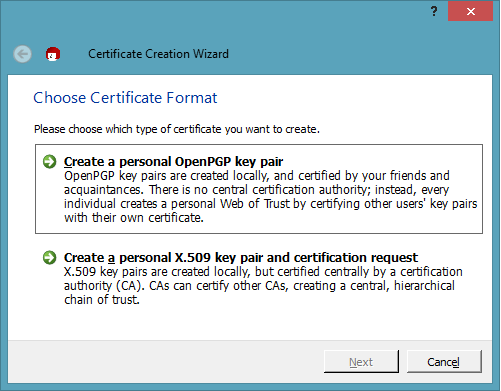
\includegraphics[width=0.8\linewidth]{pics/1.png}}
\caption{Окно создания ключа.}
\label{ris:image1}
\end{figure}

Затем введем персональную информацию \mbox(рис. {\ref{ris:image2}):} имя, почтовый адрес, комментарий. Также есть возможность задать дополнительные настройки.
\pagebreak
\begin{figure}[!h]	\center{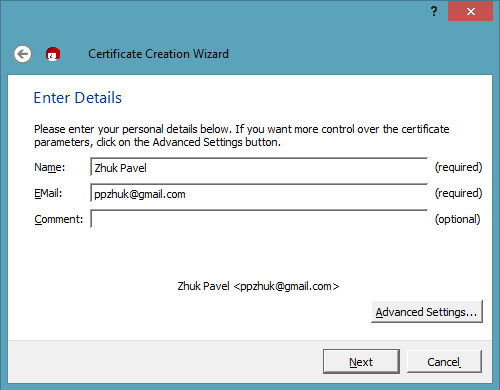
\includegraphics[width=0.8\linewidth]{pics/2.png}}
\caption{Персональные данные.}
\label{ris:image2}
\end{figure}

Далее подтверждаем ввереднную информацию \mbox{(рис. \ref{ris:image3})} и дважды вводим фразу-пароль \mbox{(рис. \ref{ris:image4})}.

\begin{figure}[!h]	\center{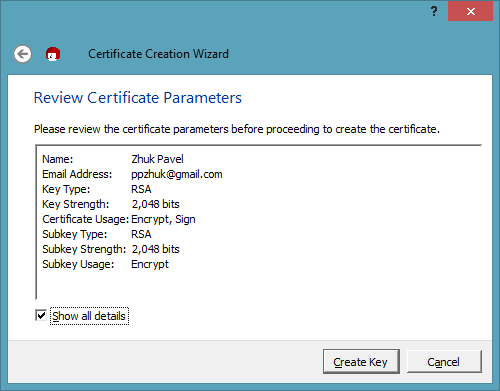
\includegraphics[width=0.8\linewidth]{pics/3.png}}
\caption{Подтверждение персональных данных.}
\label{ris:image3}
\end{figure}

\begin{figure}[!h]	\center{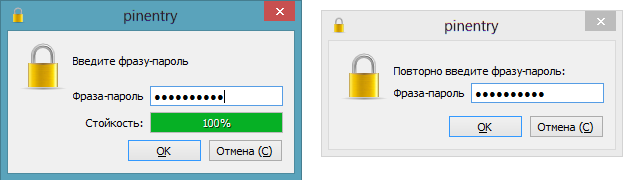
\includegraphics[width=1.1\linewidth]{pics/4.png}}
\caption{Ввод пароля.}
\label{ris:image4}
\end{figure}

\pagebreak
Ключ создан \mbox{(рис. \ref{ris:image5})}. При двойном нажатии на ключе можно посмотреть подробную информацию о нем.

\begin{figure}[!h]	\center{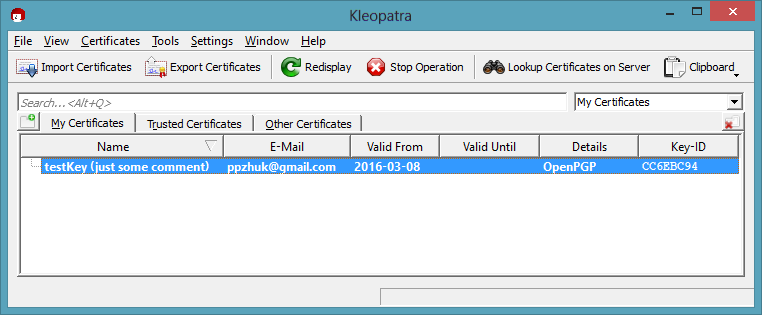
\includegraphics[width=1.3\linewidth]{pics/5.png}}
\caption{Созданный ключ.}
\label{ris:image5}
\end{figure}

\subsection{Экспортировать сертификат}
Для экспорта сертификата выберем пункт меню \textit{File $\rightarrow$ Export Certificate}. Далее выберем место сохранения сертификата и зададим название файла \mbox{(рис. \ref{ris:image6})}.

\begin{figure}[!h]	\center{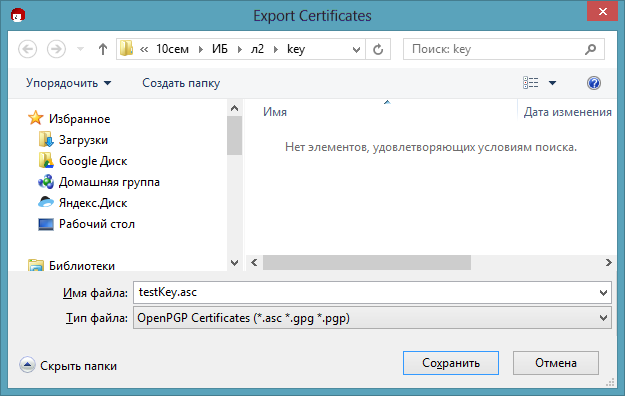
\includegraphics[width=1.1\linewidth]{pics/6.png}}
\caption{Экспорт сертификата.}
\label{ris:image6}
\end{figure}

\pagebreak
\subsection{Поставить ЭЦП на файл}
Для установки ЭЦП на файл выберем пункт меню \textit{File $\rightarrow$ Sign/Encrypt Files} и выберем нужный файл. Пусть это будет файл \textit{test.png} \mbox{(рис. \ref{ris:image7})}.

\begin{figure}[!h]	\center{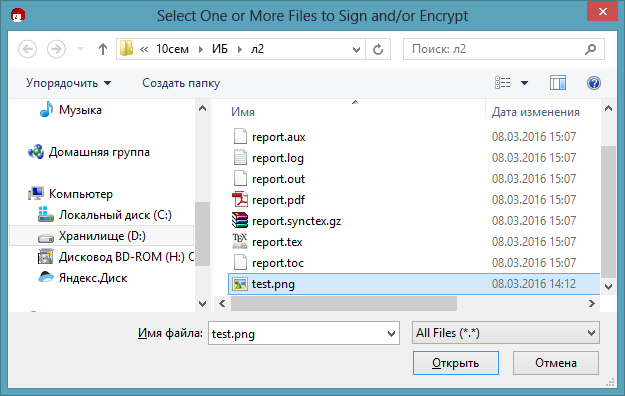
\includegraphics[width=0.9\linewidth]{pics/7.png}}
\caption{Выбор файла.}
\label{ris:image7}
\end{figure}

\pagebreak
Мы можем подписать файл (\textit{Sign}), зашифровать его (\textit{Encrypt}) или применить оба варианта вместе. Выберем вариант <<подписать файл>> \mbox{(рис. \ref{ris:image8})}.

\begin{figure}[!h]	\center{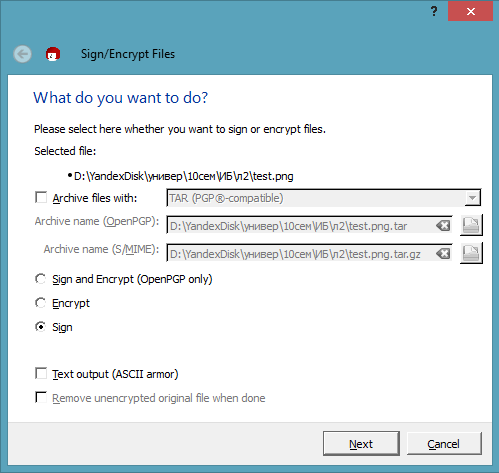
\includegraphics[width=0.8\linewidth]{pics/8.png}}
\caption{Установка ЭЦП.}
\label{ris:image8}
\end{figure}

\pagebreak
Затем выберем для подписи созданный ранее OpenPGP сертификат \mbox{(рис. \ref{ris:image9})}.

\begin{figure}[!h]	\center{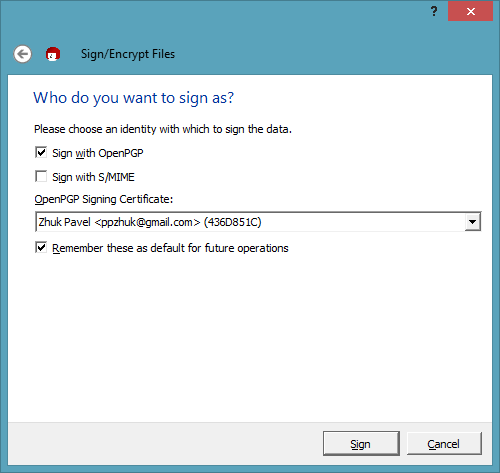
\includegraphics[width=0.8\linewidth]{pics/9.png}}
\caption{Выбор сертификата.}
\label{ris:image9}
\end{figure}

После этого необходимо ввести пароль \mbox{(рис. \ref{ris:image10})}.

\begin{figure}[!h]	\center{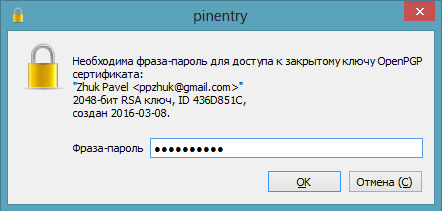
\includegraphics[width=0.9\linewidth]{pics/10.png}}
\caption{Ввод пароля.}
\label{ris:image10}
\end{figure}

И в результате получаем окно о том, что файл успешно подписан \mbox{(рис. \ref{ris:image11})}.

\begin{figure}[!h]	\center{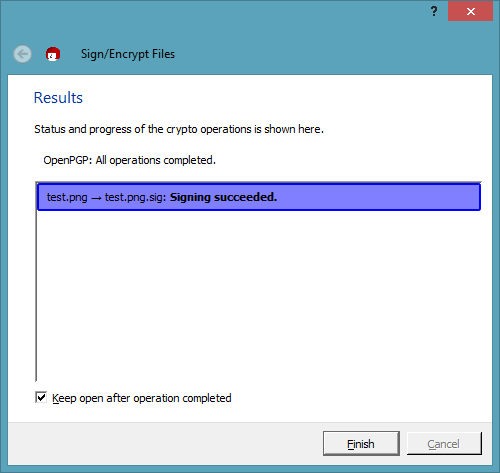
\includegraphics[width=0.8\linewidth]{pics/11.png}}
\caption{ЭЦП установлена.}
\label{ris:image11}
\end{figure}

\pagebreak
\subsection{Импортировать сертификат, подписать его}
Для импорта сертификата используется пункт меню \textit{File $\rightarrow$ Import Certificates}. Выберем данный пункт меню и затем выберем сертификат для импорта \mbox{(рис. \ref{ris:image12})}.

\begin{figure}[!h]	\center{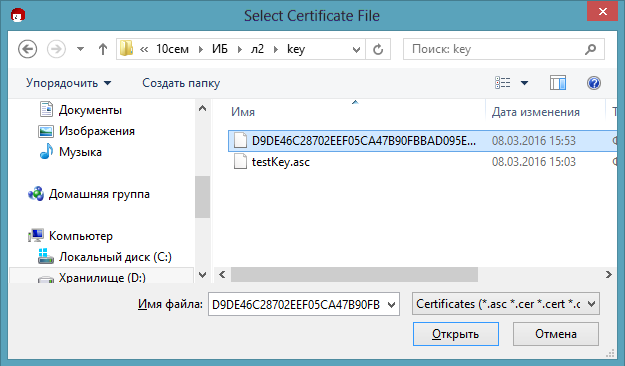
\includegraphics[width=0.8\linewidth]{pics/12.png}}
\caption{Импорт сертификата.}
\label{ris:image12}
\end{figure}

После чего отображается соответсвующее окно с результатами импорта \mbox{(рис. \ref{ris:image13})}.

\begin{figure}[!h]	\center{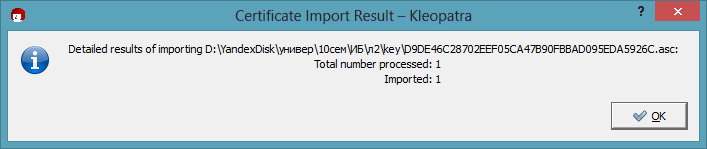
\includegraphics[width=1.2\linewidth]{pics/13.png}}
\caption{Результат импорта.}
\label{ris:image13}
\end{figure}

Подпись осуществляется аналогично предыдущему пункту. Результат показан на mbox{рисунке \ref{ris:image12})}.

\begin{figure}[!h]	\center{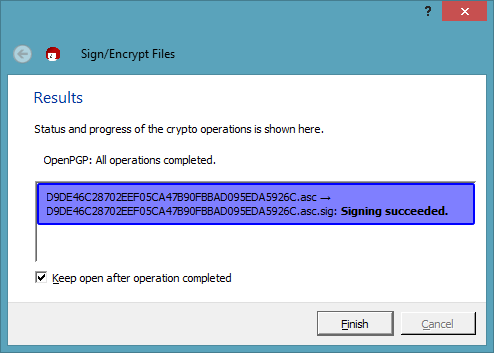
\includegraphics[width=0.8\linewidth]{pics/14.png}}
\caption{Подпись сертификата.}
\label{ris:image14}
\end{figure}

\subsection{Проверить подпись}
Для проверки подписи воспользуемся командой \textit{File $\rightarrow$ Decrypt/Verify Files} и выберем подписанный ранее сертификат (файл .asc.sig).

После нажатия на кнопку \textit{Decrypt/Verify} осуществляется проверка, которая показывает, кем была осуществлена подпись \mbox{(рис. \ref{ris:image15})}.
\begin{figure}[!h]	
\center{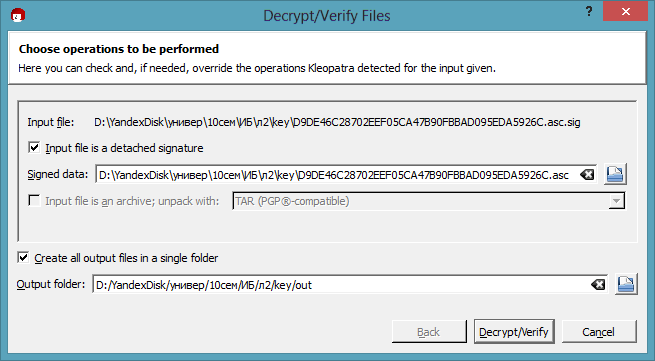
\includegraphics[width=1\linewidth]{pics/15-1.png}}
\center{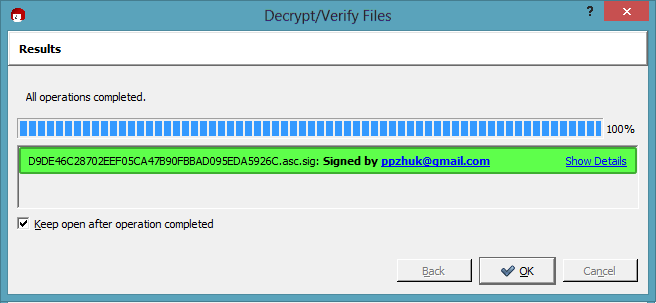
\includegraphics[width=1\linewidth]{pics/15-2.png}}
\caption{Проверка подписи сертификата.}
\label{ris:image15}
\end{figure}

\pagebreak
\subsection{Зашифровать и подписать текст чужим сертификатом.}
Был получен и импортирован способом, описанным выше, чужой сертификат под назвнием \textit{another.asc}.

Для шифрования был выбран файл \textit{testMessage.txt}, который содержит текст: \textit{There is an encrypted test message for you!}

Для шифрования и подписи файла был выбран пункт меню \textit{File $\rightarrow$ Sign/Encrypt Files}. В этот раз в настройках было выбрано \textit{Sign and Encrypt} \mbox{(рис. \ref{ris:image16})}.

\begin{figure}[!h]	\center{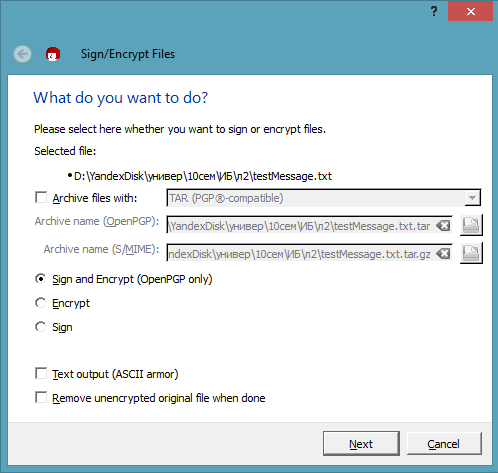
\includegraphics[width=0.8\linewidth]{pics/16.png}}
\caption{Шифрование и подпись.}
\label{ris:image16}
\end{figure}

\pagebreak
В следующем окне необходимо выбрать сертификат пользователя, для которого будет производиться шифрование \mbox{(рис. \ref{ris:image17})}. Подпись происходит, как описано выше.

\begin{figure}[!h]	\center{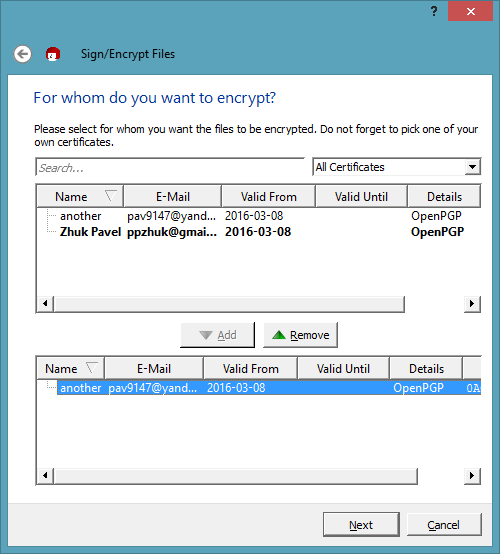
\includegraphics[width=0.8\linewidth]{pics/17.png}}
\caption{Выбор сертификата.}
\label{ris:image17}
\end{figure}

В результате получаем сообщение о том, что файл зашифрован и подписан \mbox{(рис. \ref{ris:image18})}. А также файл \textit{testMessage.txt.gpg}, который надо передать владельцу сертификата.

\begin{figure}[!h]	\center{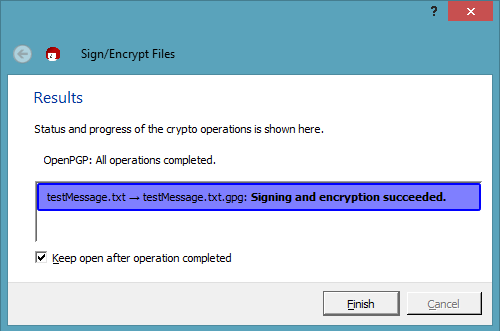
\includegraphics[width=0.8\linewidth]{pics/18.png}}
\caption{Результат.}
\label{ris:image18}
\end{figure}

\pagebreak
\subsection{Расшифровать текст зашифрованный совим сертификатом}
От коллеги был получен файл \textit{another.txt.gpg}. Расшифруем его командой \textit{File $\rightarrow$ Decrypt/Verify Files}.

В результате получился расшифрованный файл \textit{another.txt.gpg}, который содержит фразу: \textit{Hello Zhuk Pavel}.

\subsection{Потренироваться в использовании gpg через интерфейс командной строки}
Создание ключевой пары происходит с помощью ключа \textit{--gen-key}. Далее следует серия вопросов, которые помогают настроить необходимые параметры.

\begin{tabular}{|p{16cm}|}
\begin{verbatim}
C:\Users\Pavel\Desktop>gpg --gen-key
gpg (GnuPG) 2.0.29; Copyright (C) 2015 Free Software Foundation, Inc.
This is free software: you are free to change and redistribute it.
There is NO WARRANTY, to the extent permitted by law.

Выберите тип ключа:
   (1) RSA и RSA (по умолчанию)
   (2) DSA и Elgamal
   (3) DSA (только для подписи)
   (4) RSA (только для подписи)
Ваш выбор? 1
длина ключей RSA может быть от 1024 до 4096 бит.
Какой размер ключа Вам необходим? (2048)
Запрошенный размер ключа - 2048 бит
Выберите срок действия ключа.
         0 = без ограничения срока действия
      <n>  = срок действия ключа - n дней
      <n>w = срок действия ключа - n недель
      <n>m = срок действия ключа - n месяцев
      <n>y = срок действия ключа - n лет
Срок действия ключа? (0) 0
Срок действия ключа не ограничен
Все верно? (y/N) y

GnuPG необходимо составить ID пользователя в качестве идентификатора ключа.

Ваше настоящее имя: Pavel Zhuk
Адрес электронной почты: ppzhuk@gmail.com
Комментарий: The only way to survive a mad world is to embrace the madness
Вы выбрали следующий ID пользователя:
    "Pavel Zhuk (The only way to survive a mad world is to embrace the madness)
<ppzhuk@gmail.com>"

Сменить (N)Имя, (C)Комментарий, (E)Адрес или (O)Принять/(Q)Выход? O
Для защиты закрытого ключа необходима фраза-пароль.

Необходимо получить много случайных чисел. Желательно, чтобы Вы
в процессе генерации выполняли какие-то другие действия (печать
на клавиатуре, движения мыши, обращения к дискам); это даст генератору
случайных чисел больше возможностей получить достаточное количество энтропии.
gpg: ключ BF2B89B2 помечен как абсолютно доверенный.
открытый и закрытый ключи созданы и подписаны.

gpg: проверка таблицы доверия
gpg: требуется 3 с ограниченным доверием, 1 с полным, модель доверия PGP
gpg: глубина: 0  верных:   2  подписанных:   0  доверие: 0-, 0q, 0n, 0m, 0f, 2u
pub   2048R/BF2B89B2 2016-03-08
      Отпечаток ключа = 72F2 669C BA06 AC90 BD7C  31BD 65F1 66EA BF2B 89B2
uid     [абсолютное] Pavel Zhuk (The only way to survive a mad world is to embra
ce the madness) <ppzhuk@gmail.com>
sub   2048R/E3ABA2A3 2016-03-08

C:\Users\Pavel\Desktop>
\end{verbatim}
\end{tabular}\\
\newline
Вывод всех сертификатов происходит при помощи ключа  \textit{--list-keys}.\\
\newline
\begin{tabular}{|p{16cm}|}
\begin{verbatim}
C:\Users\Pavel\Desktop>gpg --list-keys
C:/Users/Pavel/AppData/Roaming/gnupg/pubring.gpg
------------------------------------------------
pub   2048R/436D851C 2016-03-08
uid     [абсолютное] Zhuk Pavel <ppzhuk@gmail.com>
sub   2048R/3FD692D3 2016-03-08

pub   2048R/0ACB54CC 2016-03-08
uid     [неизвестно] another <pav9147@yande.ru>
sub   2048R/8B2DA3AE 2016-03-08

pub   2048R/BF2B89B2 2016-03-08
uid     [абсолютное] Pavel Zhuk (The only way to survive a mad world is to embra
ce the madness) <ppzhuk@gmail.com>
sub   2048R/E3ABA2A3 2016-03-08
\end{verbatim}
\end{tabular}\\
\newline
Для симметричного шифрования файла используется ключ \textit{--symmetric}. Зашифруем файл \textit{testMessage.txt} при помощи закрытого ключа.\\
\newline
\begin{tabular}{|p{16cm}|}
\begin{verbatim}
C:\Users\Pavel\Desktop>gpg --symmetric testMessage.txt
\end{verbatim}
\end{tabular}
Получили зашифрованный файл \textit{testMessage.txt.gpg}. Для расшифровки файла необходимо использовать ключ \textit{--decrypt}.\\
\newline
\begin{tabular}{|p{16cm}|}
\begin{verbatim}
C:\Users\Pavel\Desktop>gpg --decrypt testMessage.txt.gpg
gpg: данные зашифрованы алгоритмом CAST5
gpg: зашифровано одной фразой-паролем
There is an encrypted test message for you!
gpg: ВНИМАНИЕ: целостность сообщения не защищена
\end{verbatim}
\end{tabular}\\
\newline
Также существует множество других команд, подробнее с которыми можно знакомиться в \href{https://www.gnupg.org/gph/en/manual.pdf}{The GNU Privacy Handbook}.
\section{Выводы}
Пакет \textbf{GPG4win} предоставляет удобное и простое в использовании средство для надежного шифрования файлов и органицации безопасного общения между пользователями. В данной работе были опробованы основные возможности программы. Все действия легко производятся как из командной строки, так и из графической оболочки \textbf{Kleopatra}.

\end{document}
